% Options for packages loaded elsewhere
\PassOptionsToPackage{unicode}{hyperref}
\PassOptionsToPackage{hyphens}{url}
%
\documentclass[
]{book}
\usepackage{amsmath,amssymb}
\usepackage{lmodern}
\usepackage{iftex}
\ifPDFTeX
  \usepackage[T1]{fontenc}
  \usepackage[utf8]{inputenc}
  \usepackage{textcomp} % provide euro and other symbols
\else % if luatex or xetex
  \usepackage{unicode-math}
  \defaultfontfeatures{Scale=MatchLowercase}
  \defaultfontfeatures[\rmfamily]{Ligatures=TeX,Scale=1}
\fi
% Use upquote if available, for straight quotes in verbatim environments
\IfFileExists{upquote.sty}{\usepackage{upquote}}{}
\IfFileExists{microtype.sty}{% use microtype if available
  \usepackage[]{microtype}
  \UseMicrotypeSet[protrusion]{basicmath} % disable protrusion for tt fonts
}{}
\makeatletter
\@ifundefined{KOMAClassName}{% if non-KOMA class
  \IfFileExists{parskip.sty}{%
    \usepackage{parskip}
  }{% else
    \setlength{\parindent}{0pt}
    \setlength{\parskip}{6pt plus 2pt minus 1pt}}
}{% if KOMA class
  \KOMAoptions{parskip=half}}
\makeatother
\usepackage{xcolor}
\IfFileExists{xurl.sty}{\usepackage{xurl}}{} % add URL line breaks if available
\IfFileExists{bookmark.sty}{\usepackage{bookmark}}{\usepackage{hyperref}}
\hypersetup{
  pdftitle={Accessibility Mapping for NEKRTC},
  pdfauthor={Srirama Bhamidipati; Ravi Gadepalli; Divyanka Dhok; Rupa Nandy},
  hidelinks,
  pdfcreator={LaTeX via pandoc}}
\urlstyle{same} % disable monospaced font for URLs
\usepackage[margin=1in]{geometry}
\usepackage{longtable,booktabs,array}
\usepackage{calc} % for calculating minipage widths
% Correct order of tables after \paragraph or \subparagraph
\usepackage{etoolbox}
\makeatletter
\patchcmd\longtable{\par}{\if@noskipsec\mbox{}\fi\par}{}{}
\makeatother
% Allow footnotes in longtable head/foot
\IfFileExists{footnotehyper.sty}{\usepackage{footnotehyper}}{\usepackage{footnote}}
\makesavenoteenv{longtable}
\usepackage{graphicx}
\makeatletter
\def\maxwidth{\ifdim\Gin@nat@width>\linewidth\linewidth\else\Gin@nat@width\fi}
\def\maxheight{\ifdim\Gin@nat@height>\textheight\textheight\else\Gin@nat@height\fi}
\makeatother
% Scale images if necessary, so that they will not overflow the page
% margins by default, and it is still possible to overwrite the defaults
% using explicit options in \includegraphics[width, height, ...]{}
\setkeys{Gin}{width=\maxwidth,height=\maxheight,keepaspectratio}
% Set default figure placement to htbp
\makeatletter
\def\fps@figure{htbp}
\makeatother
\setlength{\emergencystretch}{3em} % prevent overfull lines
\providecommand{\tightlist}{%
  \setlength{\itemsep}{0pt}\setlength{\parskip}{0pt}}
\setcounter{secnumdepth}{5}
\usepackage{booktabs}
\AtBeginDocument{\renewcommand{\chaptername}{}}
\usepackage{titling}
\pretitle{\begin{center} \LARGE}
\posttitle{\vskip 2cm 
\includegraphics[width=2in,height=2in]{./images/logo/Logo_UITP.png} \end{center}}
\ifLuaTeX
  \usepackage{selnolig}  % disable illegal ligatures
\fi
\usepackage[]{natbib}
\bibliographystyle{plainnat}

\title{Accessibility Mapping for NEKRTC}
\author{Srirama Bhamidipati \and Ravi Gadepalli \and Divyanka Dhok \and Rupa Nandy}
\date{2022-03-14}

\begin{document}
\maketitle

{
\setcounter{tocdepth}{1}
\tableofcontents
}
\hypertarget{introduction}{%
\chapter{Introduction}\label{introduction}}

\hypertarget{methodology-note}{%
\section{Methodology Note}\label{methodology-note}}

\begin{itemize}
\item
  Step 1: All the excel worksheets of each of the Depot we aggregated into a spatial large database with latitude and longitude values of origin, destination and the via points.
\item
  Step 2: This spatial database was then used with online routing algorithms to derive paths between origin and destinations via the intermediate points.
\item
  Step 3: Any error in the length of the paths derived and the indicated distances in the excel worksheets given by each Depot was compared and corrections were carried out to minimize the errors.
\item
  Step 4: The resulting spatial database of trips is used further to assess the accessibility of services provided in the district. The village has access to a bus service if the bus service is within 2 km of the village.
\item
  Step 5: The results for each Depot are shown in two figures: a) The geographic extent of services within Karnataka and the adjoining states, b) the accessibility with emphasis on less than 10 services a day (shades of green) and villages with no access (red)
\end{itemize}

\hypertarget{kalaburagi}{%
\chapter{Kalaburagi}\label{kalaburagi}}

\begin{itemize}
\tightlist
\item
  In total 2344 trips were mapped for Kalaburagi.
\item
  These trips cover about 67 percent of villages in the district.
\item
  A total of 333 villages are not covered by any bus service.
\item
  The spatial distribution of trips are shown in figure \ref{fig:routesKala}
\item
  The spatial distribution of villages covered and villages not covered by the bus services are shown in figure \ref{fig:accessKala}
\end{itemize}

\begin{figure}
\centering
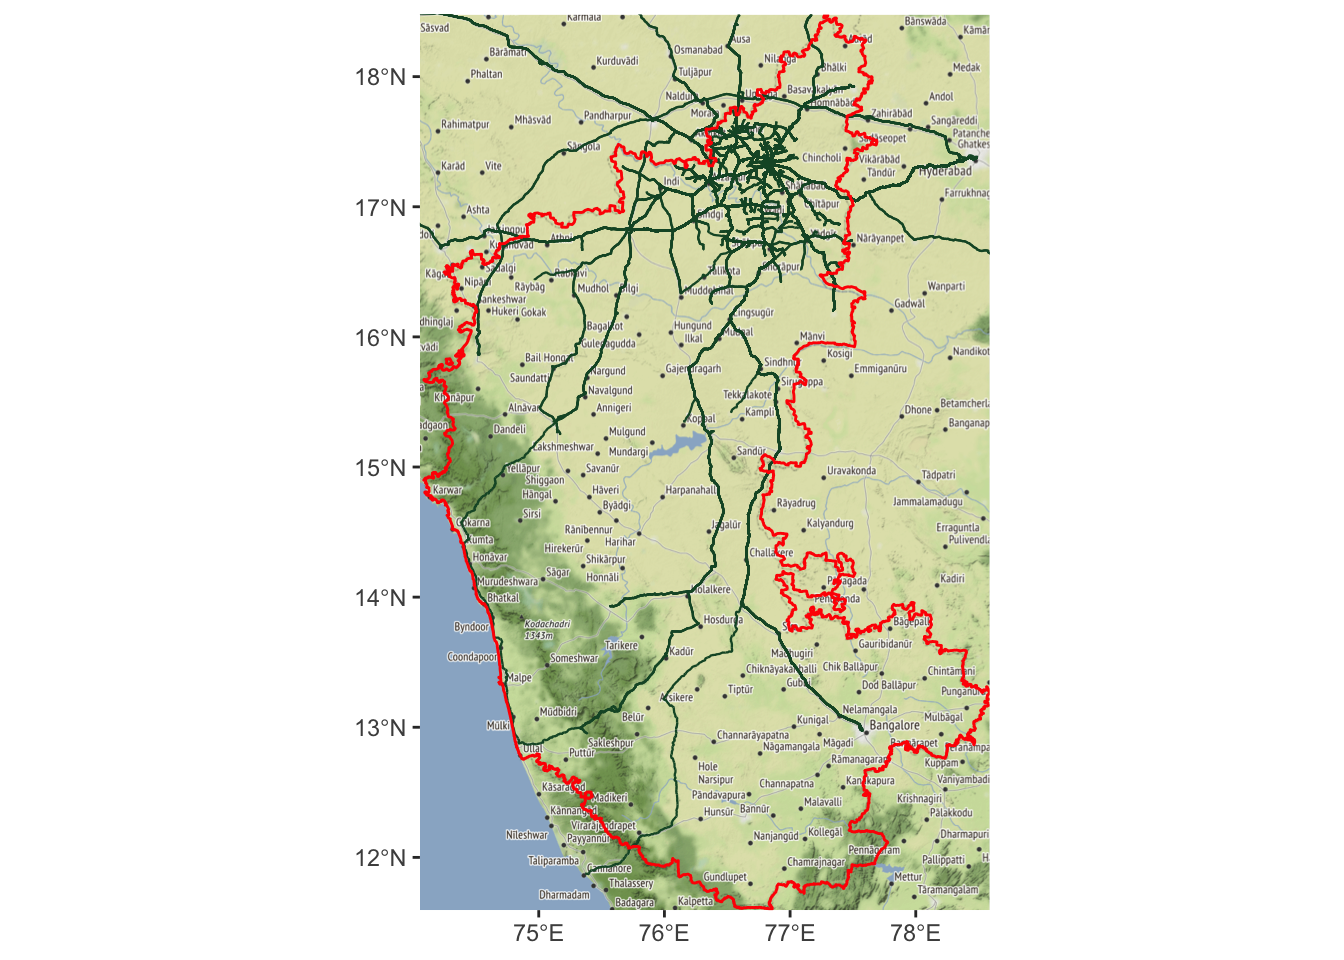
\includegraphics{NEKRTC_spatial_mapping_files/figure-latex/routesKala-1.pdf}
\caption{\label{fig:routesKala}Extent of services from Kalaburagi}
\end{figure}

\begin{figure}
\centering
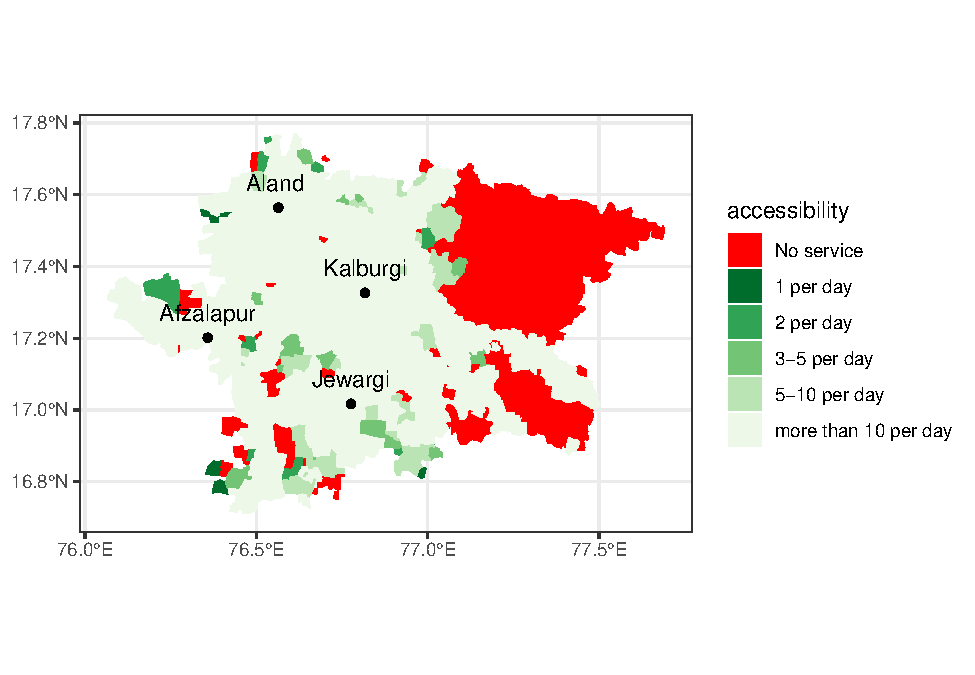
\includegraphics{NEKRTC_spatial_mapping_files/figure-latex/accessKala-1.pdf}
\caption{\label{fig:accessKala}Accessibility in Kalaburagi}
\end{figure}

\hypertarget{koppal}{%
\chapter{Koppal}\label{koppal}}

\begin{itemize}
\tightlist
\item
  In total 1970 trips were mapped for Koppal
\item
  These trips cover about 95 percent of villages in the district.
\item
  A total of 38 villages are not covered by any bus service.
\item
  The spatial distribution of trips are shown in figure \ref{fig:routesKopa}
\item
  The spatial distribution of villages covered and villages not covered by the bus services are shown in figure \ref{fig:accessKoppa}
\end{itemize}

\begin{figure}
\centering
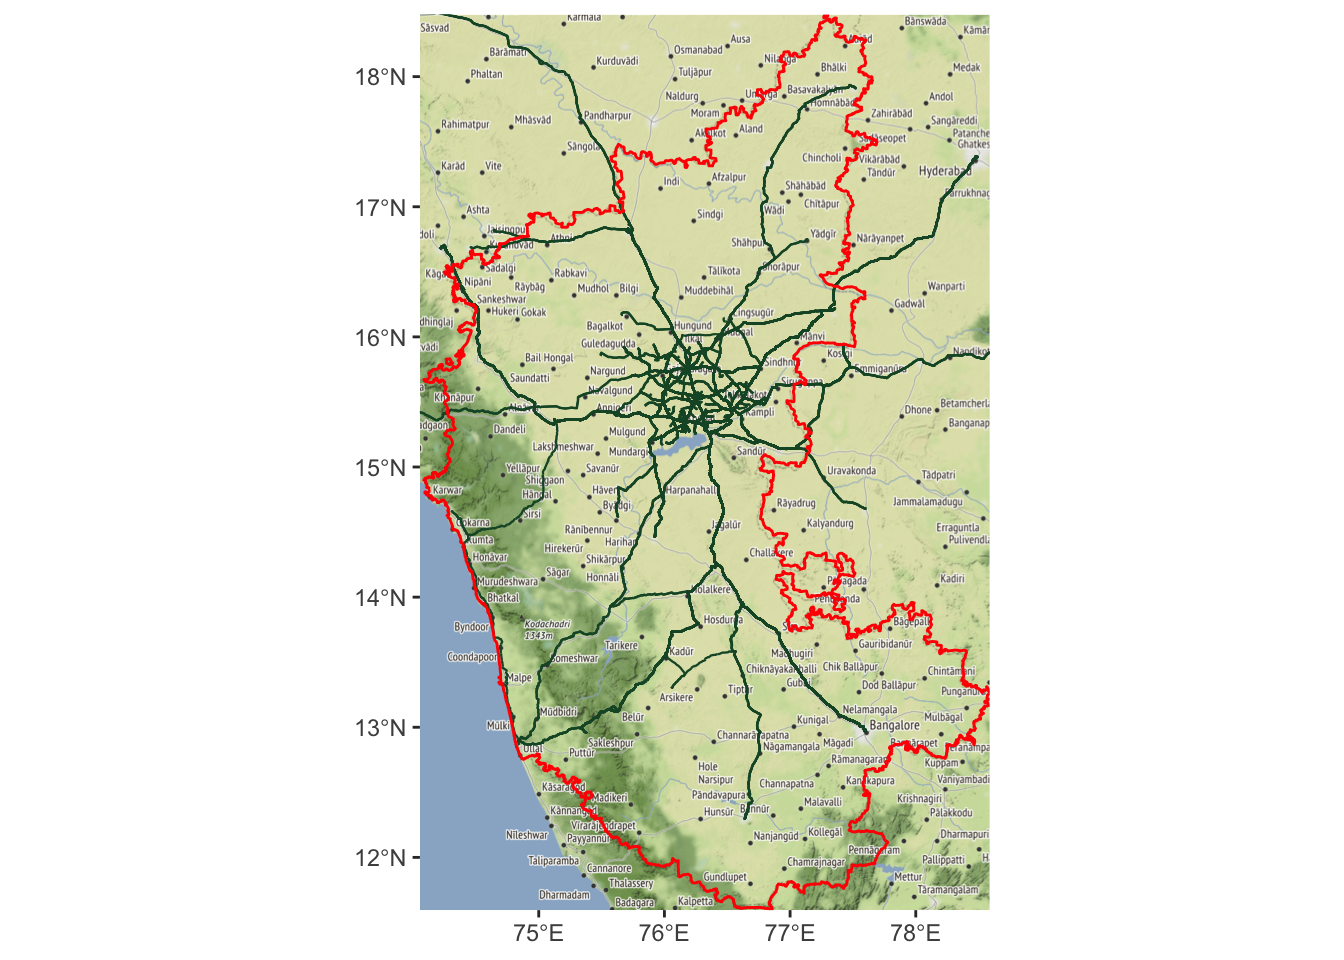
\includegraphics{NEKRTC_spatial_mapping_files/figure-latex/routesKopa-1.pdf}
\caption{\label{fig:routesKopa}Extent of services from Koppal}
\end{figure}

\begin{figure}
\centering
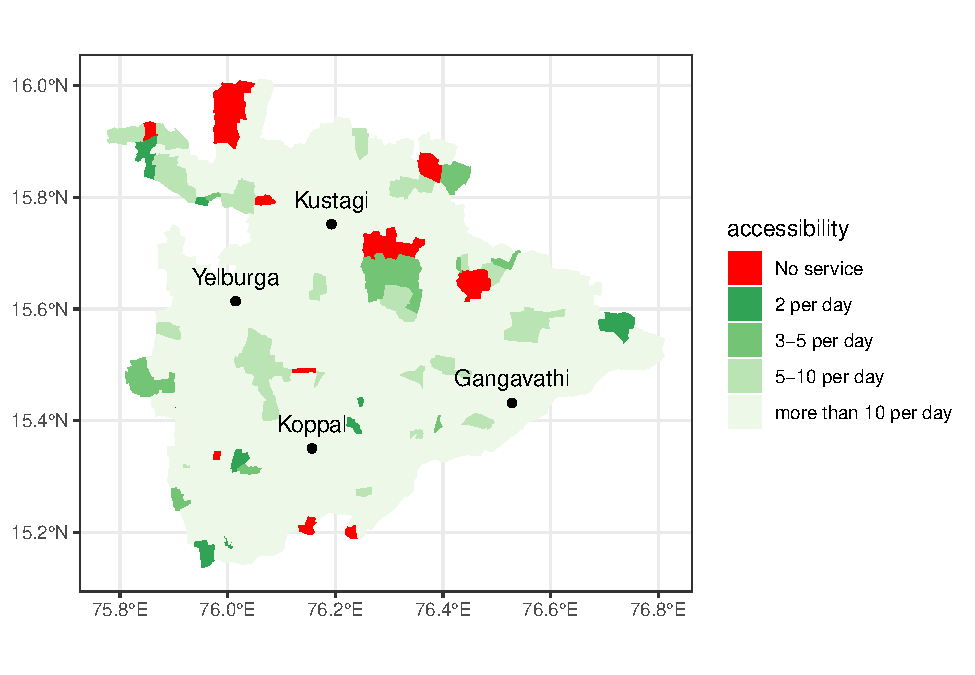
\includegraphics{NEKRTC_spatial_mapping_files/figure-latex/accessKoppa-1.pdf}
\caption{\label{fig:accessKoppa}Accessibility in Koppal}
\end{figure}

\hypertarget{yadgiri}{%
\chapter{Yadgiri}\label{yadgiri}}

\begin{itemize}
\tightlist
\item
  In total 1418 trips were mapped for Yadgiri
\item
  These trips cover about 90 percent of villages in the district.
\item
  A total of 59 villages are not covered by any bus service.
\item
  The spatial distribution of trips are shown in figure \ref{fig:routesYad}
\item
  The spatial distribution of villages covered and villages not covered by the bus services are shown in figure \ref{fig:accessYad}
\end{itemize}

\begin{figure}
\centering
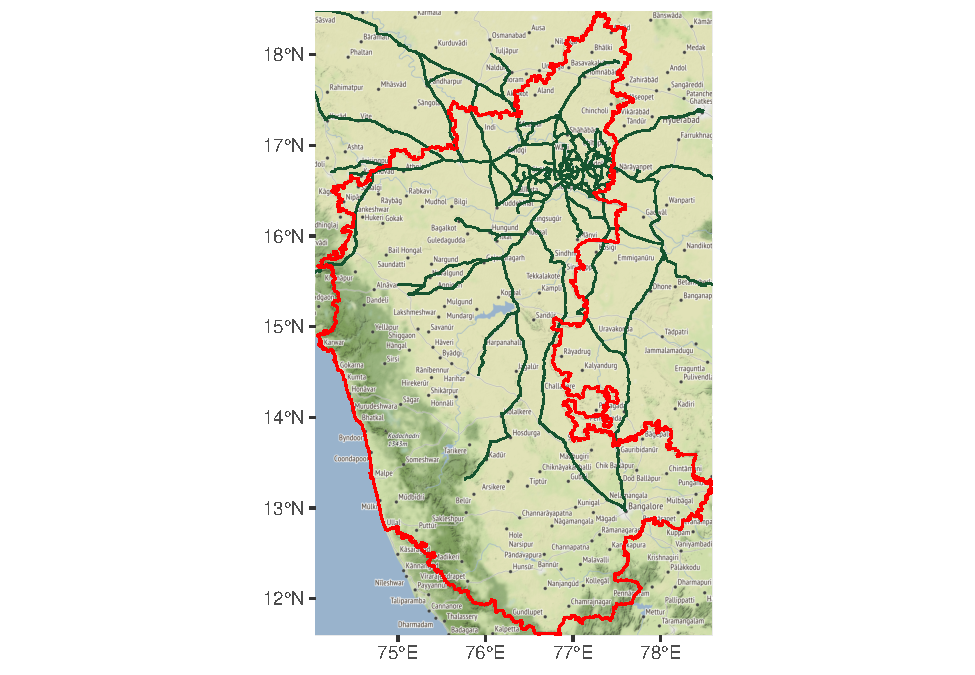
\includegraphics{NEKRTC_spatial_mapping_files/figure-latex/routesYad-1.pdf}
\caption{\label{fig:routesYad}Extent of services from Yadgir}
\end{figure}

\begin{figure}
\centering
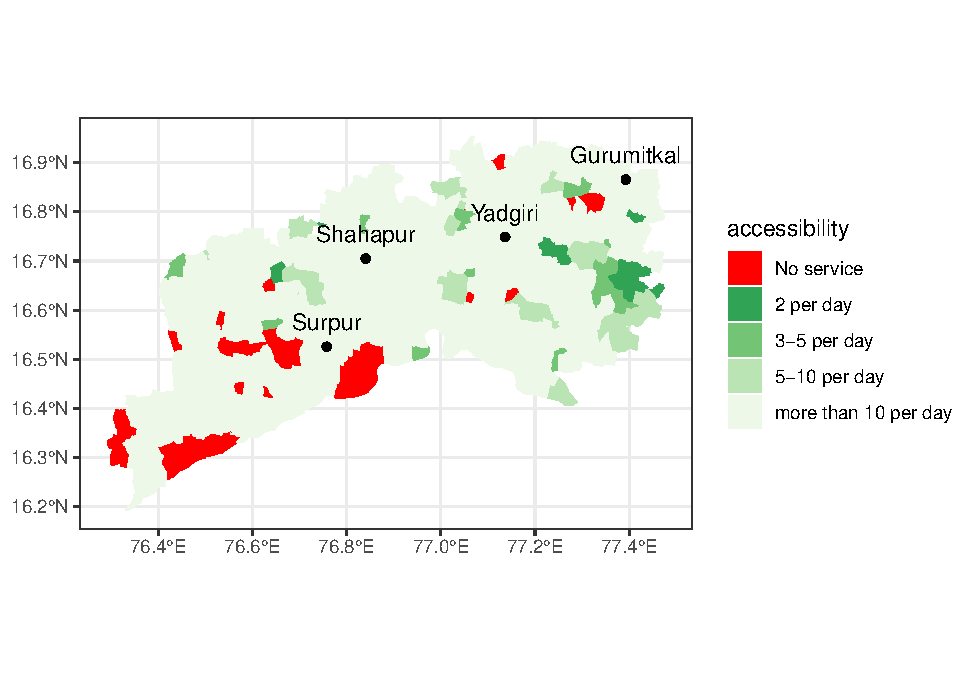
\includegraphics{NEKRTC_spatial_mapping_files/figure-latex/accessYad-1.pdf}
\caption{\label{fig:accessYad}Accessibility in Yadgiri}
\end{figure}

\hypertarget{hospete}{%
\chapter{Hospete}\label{hospete}}

\begin{itemize}
\tightlist
\item
  In total 1880 trips were mapped for Hospete
\item
  These trips cover about 76 percent of villages in the district.
\item
  A total of 181 villages are not covered by any bus service.
\item
  The spatial distribution of trips are shown in figure \ref{fig:routesHos}
\item
  The spatial distribution of villages covered and villages not covered by the bus services are shown in figure \ref{fig:accessHos}
\end{itemize}

\begin{figure}
\centering
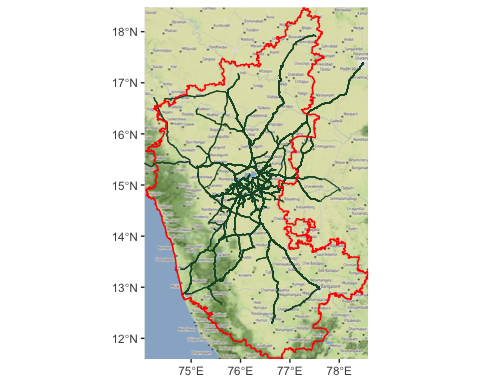
\includegraphics{NEKRTC_spatial_mapping_files/figure-latex/routesHos-1.pdf}
\caption{\label{fig:routesHos}Extent of services from Hospete}
\end{figure}

\begin{figure}
\centering
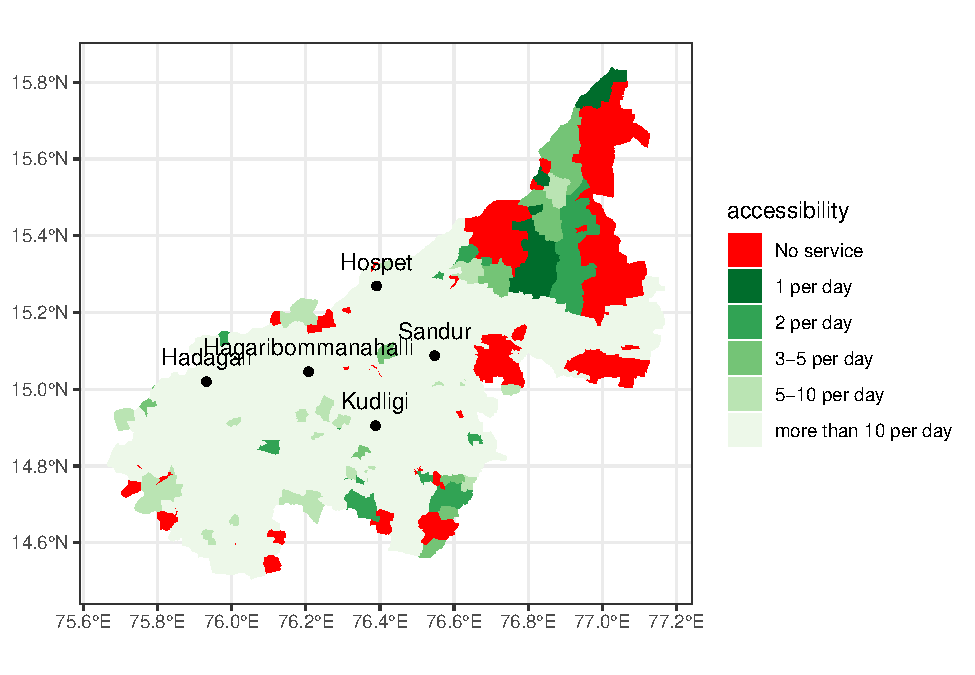
\includegraphics{NEKRTC_spatial_mapping_files/figure-latex/accessHos-1.pdf}
\caption{\label{fig:accessHos}Accessibility in Hospete}
\end{figure}

\hypertarget{bidar}{%
\chapter{Bidar}\label{bidar}}

\begin{itemize}
\tightlist
\item
  In total 2980 trips were mapped for Bidar
\item
  These trips cover about 95 percent of villages in the district.
\item
  A total of 39 villages are not covered by any bus service.
\item
  The spatial distribution of trips are shown in figure \ref{fig:routesBid}
\item
  The spatial distribution of villages covered and villages not covered by the bus services are shown in figure \ref{fig:accessBid}
\end{itemize}

\begin{figure}
\centering
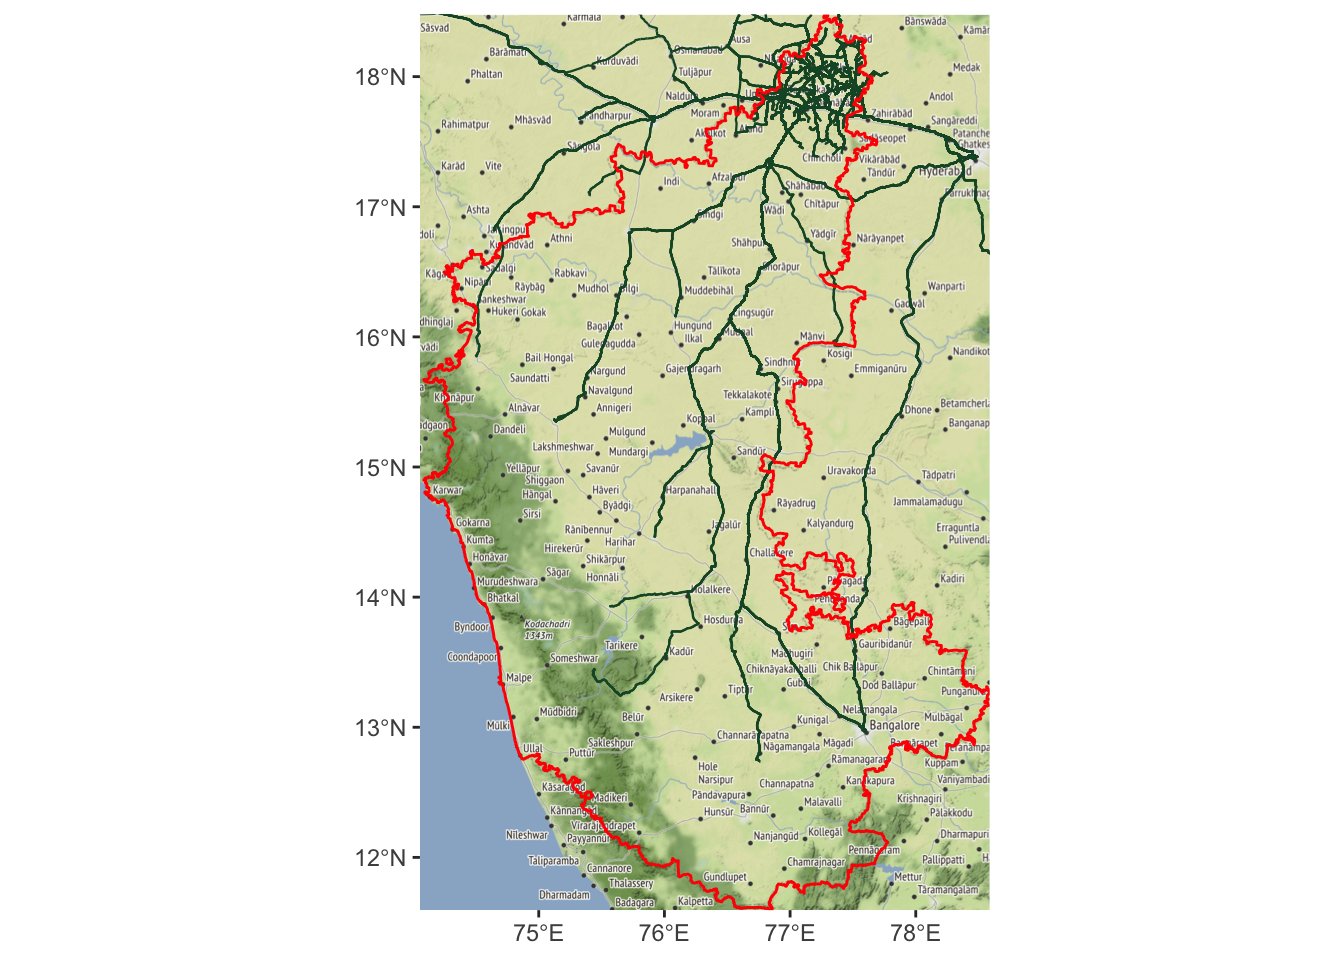
\includegraphics{NEKRTC_spatial_mapping_files/figure-latex/routesBid-1.pdf}
\caption{\label{fig:routesBid}Extent of services from Bidar}
\end{figure}

\begin{figure}
\centering
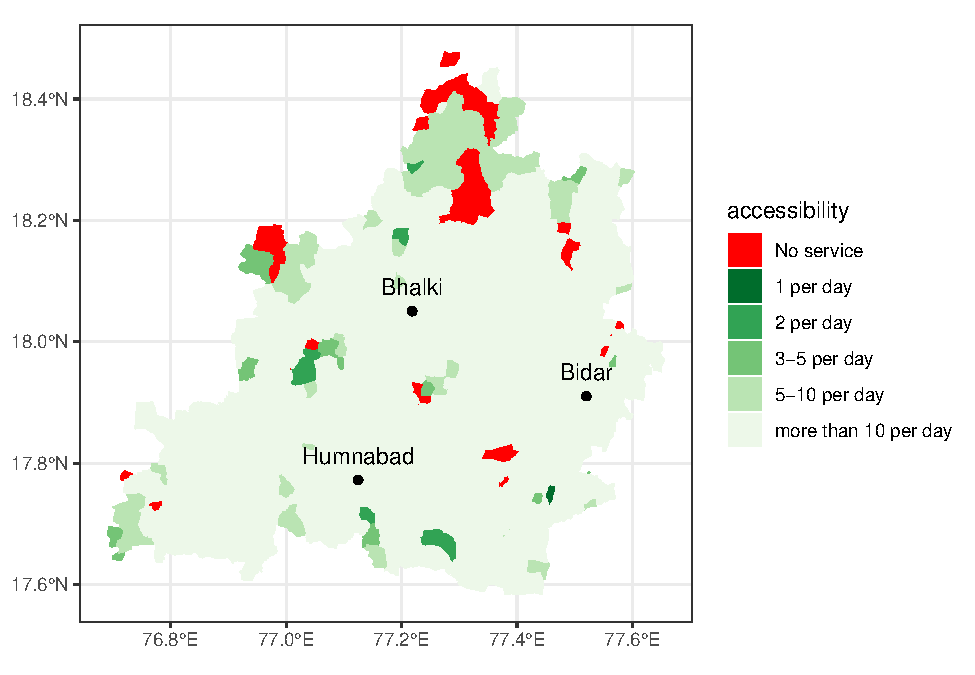
\includegraphics{NEKRTC_spatial_mapping_files/figure-latex/accessBid-1.pdf}
\caption{\label{fig:accessBid}Accessibility in Bidar}
\end{figure}

  \bibliography{book.bib,packages.bib}

\end{document}
